\section{Backend}
\rhead{Backend}
\subsection{Használt technológiák}
A backend megírásánál az egyszerűségre és a későbbi könnyebb felhasználhatóságra törekedtünk, így esett választásunk a Go-MongoDB stack-re.
\subsubsection{MongoDB}
A \emph{MongoDB}\footnote{\url{https://www.mongodb.com/}} egy NoSQL adatbázis, amely azt jelenti, hogy táblák és sorok helyett egy JSON szerű struktúrában tárolja el az adatokat.
Ennek számos előnye és hátránya is van.

\begin{samepage}
  \noindent Előnyei:
  \begin{itemize}
    \item Egyszerű feltöltés/letöltés a JSON szerű formátum miatt
    \item Nem szükséges előre felépíteni az adatbázis struktúráját
    \item Frissítések valós-idejű figyelése
  \end{itemize}

  \noindent Hátrányai:
  \begin{itemize}
    \item Ritkábban használt
    \item Átlagoshoz képest komplexebb lekérdezések
    \item Sémának való megfelelés nem ellenőrzött
    \item Kevésbé rendezett, mint a relációs adatbázisok
  \end{itemize}
\end{samepage}

Az említett valós-idejű figyelés, amely egy felhasználó projektjeinek folyamatos frissítéséhez szükséges, csak replica set esetén működik, tehát akkor ha a szerver be van állítva a megosztott munkára.
\subsubsection{Go}
A stack másik tagja, a \emph{Go}\footnote{\url{https://golang.org/}} egy programozás nyelv, amelyet a Google fejlesztett ki. A cél egy átlátható, egyszerű nyelv készítése volt, amely helyettesítheti a halom másik náluk használt programozási nyelvet. \cite{golang}

\begin{samepage}
  \noindent Előnyei:
  \begin{itemize}
    \item Típusos, így kisebb az esélye a hibáknak
    \item Erős beépített webfejlesztési (HTTP, sablonok stb.) könyvtárak
    \item Egyszerű párhuzamos futtatás \emph{Goroutine}-okkal és csatornákkal
    \item Fordított, de szemétgyűjtős

  \end{itemize}
\end{samepage}

\begin{samepage}
  \noindent Hátrányai:
  \begin{itemize}
    \item Adatfeldolgozási függvényekben hiányos
    \item Generikusok hiánya
    \item Frusztrálóan bő szavú hibakezelés
  \end{itemize}
\end{samepage}

Az e-mail rendszerhez a beépített NET/SMTP könyvtárat használtuk az üzenetek elküldéséhez, illetve a HTML/template könyvtárat az üzenetek tartalmának kitöltéséhez.

A fejlesztésben sokat segített a \emph{Gorilla} könyvtár, amely az alapértelmezett HTTP könyvtárat egészíti ki további hasznos funkciókkal.
Például middleware támogatással, metódus korlátozással, URL-be helyezett paraméterekkel stb.

\subsection{Szolgáltatások méretezése}
A \emph{docker-compose} fájlban található \emph{Traefik}\footnote{\url{https://traefik.io/traefik/}} két fő feladatot lát el:

\begin{samepage}
  \begin{itemize}
    \item Statikus frontend fájlok és a Backend API egy végpontra helyezése
    \item Automatikus terheléselosztás
  \end{itemize}
\end{samepage}

A \emph{Traefik} integrálja magát a \emph{Docker}-be, és így látja, ha egy szolgáltatásból több fut, és el tudja közöttük osztani a terhet.

Ha szeretnénk egy szolgáltatást méretezni, akkor a \emph{docker-compose} parancsot kell lefuttatnunk, a következő parancsok egyikével:

\begin{itemize}
  \item Statikus fájl szerver méretezése
        \begin{lstlisting}[language=bash]
        $ docker-compose up --scale frontend=<DARAB>\end{lstlisting}
  \item Backend szerver méretezése
        \begin{lstlisting}[language=bash]
        $ docker-compose up --scale backend=<DARAB>\end{lstlisting}
\end{itemize}

\subsection{Adatbázis modell}

Az adatokat a \emph{MongoDB} nevű adatbázis-kezelőben tároljuk el, amely NoSQL technológiára épül, így teljesen más struktúrát követel, mint egy relációs adatbázis. Míg a relációs adatbázisok egy gráf szerkezetet használnak, addig a \emph{MongoDB} egy fastruktúrát.

\begin{figure}[H]
  \centering
  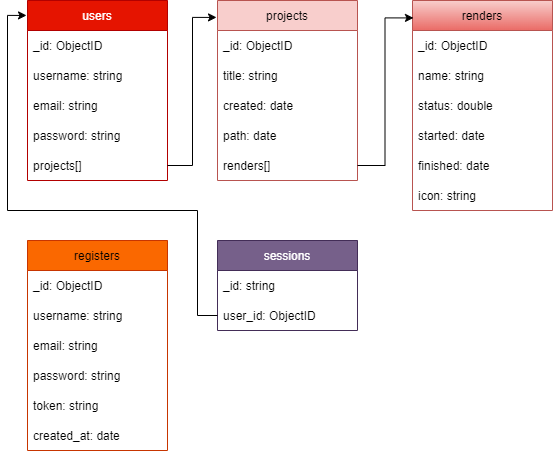
\includegraphics[width=.7\textwidth]{parts/developer-documentation/backend/images/model.png}
  \caption{Az Archytex adatbázis modellje}
\end{figure}


Három különböző dokumentumtípust különböztetünk meg:
\begin{itemize}
  \item users

        A regisztrált és regisztrációjukat megerősített felhasználók listája
  \item registers

        A regisztrált, de még nem megerősített felhasználók listája
  \item sessions

        A jelenleg belépett felhasználók listája
\end{itemize}

\pagebreak

\subsubsection{Users dokumentum}
\begin{itemize}
  \item \_id

        Típus: ObjectID

        Leírás: A \emph{MongoDB} által generált egyedi azonosító
  \item username

        Típus: string

        Leírás: A felhasználó választott neve
  \item email
        Típus: string

        Leírás: A felhasználó e-mail címe
  \item password

        Típus: string

        Leírás: A felhasználó jelszavának ellenőrzésére szolgáló kriptográfiai karakterlánc
  \item projects

        Típus: Tömb, Lásd lent

        Leírás: A felhasználó projektjeinek listája
\end{itemize}

\subsubsection{Projects al-dokumentum}

\begin{itemize}
  \item \_id

        Típus: ObjectID

        Leírás: A \emph{MongoDB} által generált egyedi azonosító
  \item title

        Típus: string

        Leírás: A projekt címe
  \item created

        Típus: date

        Leírás: A projekt létrehozásának időpontja
  \item path

        Típus: string

        Leírás: A szerver fájlrendszerében lévő ASCN fájl neve
  \item renders

        Típus: Tömb, Lásd lent

        Leírás: A projekthez tartozó renderek listája
\end{itemize}
\subsubsection{Renders al-al-dokumentum}

\begin{itemize}
  \item \_id

        Típus: ObjectID

        Leírás: A \emph{MongoDB} által generált egyedi azonosító
  \item name

        Típus: string

        Leírás: A render neve
  \item status

        Típus: double

        Leírás: A render elkészültségének jelenlegi állapota, 0-tól 1-ig tartó valós szám
  \item started

        Típus: date

        Leírás: A render munka elküldésének időpontja
  \item finished

        Típus: date

        Leírás: A render befejezésének időpontja
  \item icon

        Típus: string

        Leírás: A szerver fájlrendszerében lévő képfájl neve
\end{itemize}

\subsubsection{Registers dokumentum}

\begin{itemize}
  \item \_id

        Típus: ObjectID

        Leírás: A \emph{MongoDB} által generált egyedi azonosító
  \item username

        Típus: string

        Leírás: A felhasználó választott neve
  \item email

        Típus: string

        Leírás: A felhasználó ímélcíme
  \item password

        Típus: string

        Leírás: A felhasználó jelszavának ellenőrzésére szolgáló kriptográfiai karakterlánc
  \item token

        Típus: string

        Leírás: A regisztráció megerősítéséhez szükséges egyszer használatos azonosító
  \item created\_at

        Típus: date

        Leírás: A regisztrációs szándék beadásának időpontja. Segítségével létre lehet hozni olyan indexet, ami a kérelmet törli bizonyos idő lejárta után.
\end{itemize}
\subsubsection{Sessions dokumentum}

\begin{itemize}
  \item \_id

        Típus: string (fontos)

        Leírás: Kriptográfiailag generált karakterlánc, amely a felhasználót azonosítja bejelentkezés után
  \item user\_id

        Típus: ObjectID

        Leírás: A felhasználó egyedi azonosítója
\end{itemize}


\subsection{Backend .env fájl}

A backend konfigurálását egy .env fájl segítségével lehet megtenni. Ha a Docker környezetet használjuk, ezt a fájlt nem szükséges kitölteni, ahhoz külön .env fájl tartozik.

Szükséges konfigurációs paraméterek:
\begin{itemize}
  \item SMTP beállítások
        \subitem SMTP\_SERVER

        SMTP szerver címe
        \subitem SMTP\_ADDRESS

        SMTP szerveren lévő e-mail cím
        \subitem SMTP\_PASSWORD

        Az előbb használt ímélcímhez tartozó jelszó
        \subitem SMTP\_PASSWORD

        Az előbb használt ímélcímhez tartozó jelszó
  \item MongoDB beállítások
        \subitem MONGO\_URI

        MongoDB-hez való csatlakozáshoz szükséges URI
        \subitem MONGO\_DB

        MongoDB adatbázis neve
  \item RabbitMQ beállítások
        \subitem AMQP\_ADDR

        AMQP (RabbitMQ)-hez való csatlakozáshoz szükséges URI
  \item Redis beállítások
        \subitem REDIS\_ADDR

        Redis-hez való csatlakozáshoz szükséges URI
  \item Egyéb
        \subitem PROJECTS\_PATH

        Projektfájlok és renderek tárolására elkülönített mappa elérési útja
        \subitem PORT

        Szerver portja
        \subitem DOMAIN

        A szerver távoli címe, amelyet a megerősítő ímélben használunk
        \subitem CAPTCHA\_SECRET

        ReCaptcha szolgáltatásból érkező titkos kulcs
\end{itemize}

Példa:

\begin{lstlisting}
PORT=8080
MONGO_URI=mongodb://localhost:27017
MONGO_DB=archytex
SMTP_SERVER=smtp.gmail.com:587
SMTP_ADDRESS=archytex@gmail.com
SMTP_PASSWORD=password
AMQP_ADDR=amqp://127.0.0.1:5672
REDIS_ADDR=127.0.0.1:6379
CAPTCHA_SECRET=SECRETSECRETSECRETSECRETSECRETSECRET
PROJECTS_PATH=F:/archytex_storage
DOMAIN=https://archytex.me
\end{lstlisting}

\subsection{HTTP dokumentáció}
A HTTP végpontok dokumentációja elérhető OpenAPI formátumban a repo gyökérkönyvtárában \emph{openapi.yml} néven.

\subsection{WebSocket dokumentáció}
A /api/ws végponton elérhető egy WebSocket szolgáltatás, amely a projektek listájának frissítésére szolgál. A lista bármilyen változása esetén újraküldi a kliens felé a lista összes elemét, JSON formátumban kódolva a \emph{projects} kulcs alatt.

A WebSocket protokoll nem engedélyezi az egyéni HTTP fejlécek használatát, így a felhasználó azonosítására nem használható az \emph{Authorization} fejléc. A probléma megoldásának érdekében a szerver addig nem küld semmilyen adatot a kliensnek, ameddig a kliens el nem küldi a jelenleg használt session azonosítóján JSON karakterláncként kódolva.

\pagebreak

Szerver felől érkező üzenet példa:
\begin{lstlisting}
{
  "projects": [
    {
      "id": "62321eef021ec8e9e88e0e0b",
      "title": "test",
      "created": "2022-03-16T17:31:27.548Z",
      "renders": [
        {
          "id": "623474fcbcbcfc406f415db2",
          "name": "test-1",
          "status": 0,
          "started": "2022-03-18T12:03:08.085Z",
          "finished": "2022-03-18T12:04:08.085Z",
          "icon": "62347542b583efa2bab25a90"
        },
        {
          "id": "623474fdbcbcfc406f415db3",
          "name": "test-2",
          "status": 0,
          "started": "2022-03-18T12:03:09.313Z",
          "finished": null,
          "icon": ""
        }
      ]
    }
  ]
}
\end{lstlisting}